\documentclass[10pt,twocolumn,letterpaper]{article}

\usepackage{cvpr}
\usepackage[utf8]{inputenc}
\usepackage{gensymb}
\usepackage{graphicx}
\graphicspath{ {imgs/} }
\usepackage{float}

\cvprfinalcopy
\def\cvprPaperID{a1700831} % *** Enter the CVPR Paper ID here


% begin of document
\begin{document}
\title{Assignment 1 - Method for Creating Mosaics by Brown and Lowe}
\author{Yuanzhong Xia\\
University of Adelaide\\
SA, Australia\\
{\tt\small a1700831@student.adelaide.edu.au}
}
\maketitle

% abstract
\begin{abstract}
This is the assignment 1 report, describing and testing a method for creating panorama from a set of smaller images.
The related codes are using Java binding version of OpenCV, and it contains my partial implemented improved method, which is used to test my hypothesis and improvements.
\end{abstract}


\section{The Problem}
The problem is to stitch many images of different small areas into a large panorama image.
However, the images standing for small areas often have lots of issues when stitching.
The images can have different rotations, scales, affine, projective transformations, photometric problems, moving objects and so on.

To stitch the images into a large panorama, the method must overcome most of the issues above,
and the most important thing is to make sure the image look normal and less noticeable.


\section{Brown and Lowe's Method}
The method is being discovered for a long time. But none of them can perform better than Brown and Lowe's method \cite{origin}.
Brown and Lowe's method can overcome the issues caused by variant orientations, zoomings, and do color corrections and moving object detection to some extend.

The method is based on invariant features appearing in multiple images. If the combination of invariant features in two images match with each other,
they can be stitched together by superposing the matching features, and vise versa, they cannot. 

\subsection{Description}
The psedocodes on the paper have already show the outline the stitching algorithm.
Here are the more detailed description:
\begin{enumerate}
%% todo: add some numeric analysis
    \item Read all input images, \textit{(if the number of images is less than two, \textbf{fail} because one image does not need to be stitched.)}
    \item Extract SIFT \cite{sift} features from all images,
    \item Store $k$-nearest neighbor features using a k-d tree \cite{knn}, \textit{(increase the accuracy for feature matching.)}
    \item Match the potential images using RANSAC \cite{ransac}, and verify them using a probabilistic model %%todo cite , \textit{(if the probability is not high enough, and there isn't any image can be stitched with this image, \textbf{fail})}
    \item 
\end{enumerate}

This is the description.% idea of simulating a wider view filed len

\subsection{Limitation and Improvements}
Analyse the limitation and improvements.

Brown and Lowe's method uses the feature that the images are assumed to be captured by a centric camera,
because in the ``straightening'' method, they ignore the case that the camera is not moved horizontally.
They use a camera position detection idea to straighten the long curved image into long stright image.
Therefore, if the images are taken horizontally, they will be unable to be stitched together in that no two images can match by features.

% improvements


\section{Testing}
% non-free SIFT
\textit{(the OpenCV implementation uses speeded up robust features (SURF) \cite{surf} to generate the feature)}



At the beginning, I tried to experiment in a measurable way, which can produce some mathematical benchmark results. Here are the steps:
\begin{enumerate}
    \item Select a long image, \textit{(produce the images from panorama.)}
    \item Draw a horizontal line with 2 pixel width from left most to right most in vertical center, \textit{(create a baseline for benchmark, but the line should not affect the extraccted feature set of the original images.)}
    \item Split the image into three images: left, middle and right (each adjacent two images have 30\% shared area, and have same width), \textit{(make it simple, use only three images.)}
    \item Distort the left image to make the length of its left edge is two times larger than the length of its right edge, \textit{(simulate the projection effect.)}
    \item Distort the right image to make the length of its right edge is two times large than the length of its left edge, \textit{(simulate the projection effect.)}
    \item Rotate the left image for 30\degree clockwise, \textit{(just a random value to test , because idealy, the feature matching algorithm can match SIFT feature in any orientation.)}
    \item Zoom out to fit the rectangle window, \textit{(the image should still be a rectangle.)}
    \item Stitch them with Brown and Lowe's methods, \textit{(do stitching.)}
    \item Measure the following values, \textit{(metric test.)} 
    \begin{itemize}
        \item The average running time with 30 repeatitions in millisecond,
        \item The mean square error (MSE) of the baseline's curvity,
        \item The minimum distance between each two baselines' endpoints in pixel, larger than 0 if the three baseline segments (each image has one) are not stitched together,
    \end{itemize}
\end{enumerate}

% but

\begin{figure}[t]
    \begin{center}
        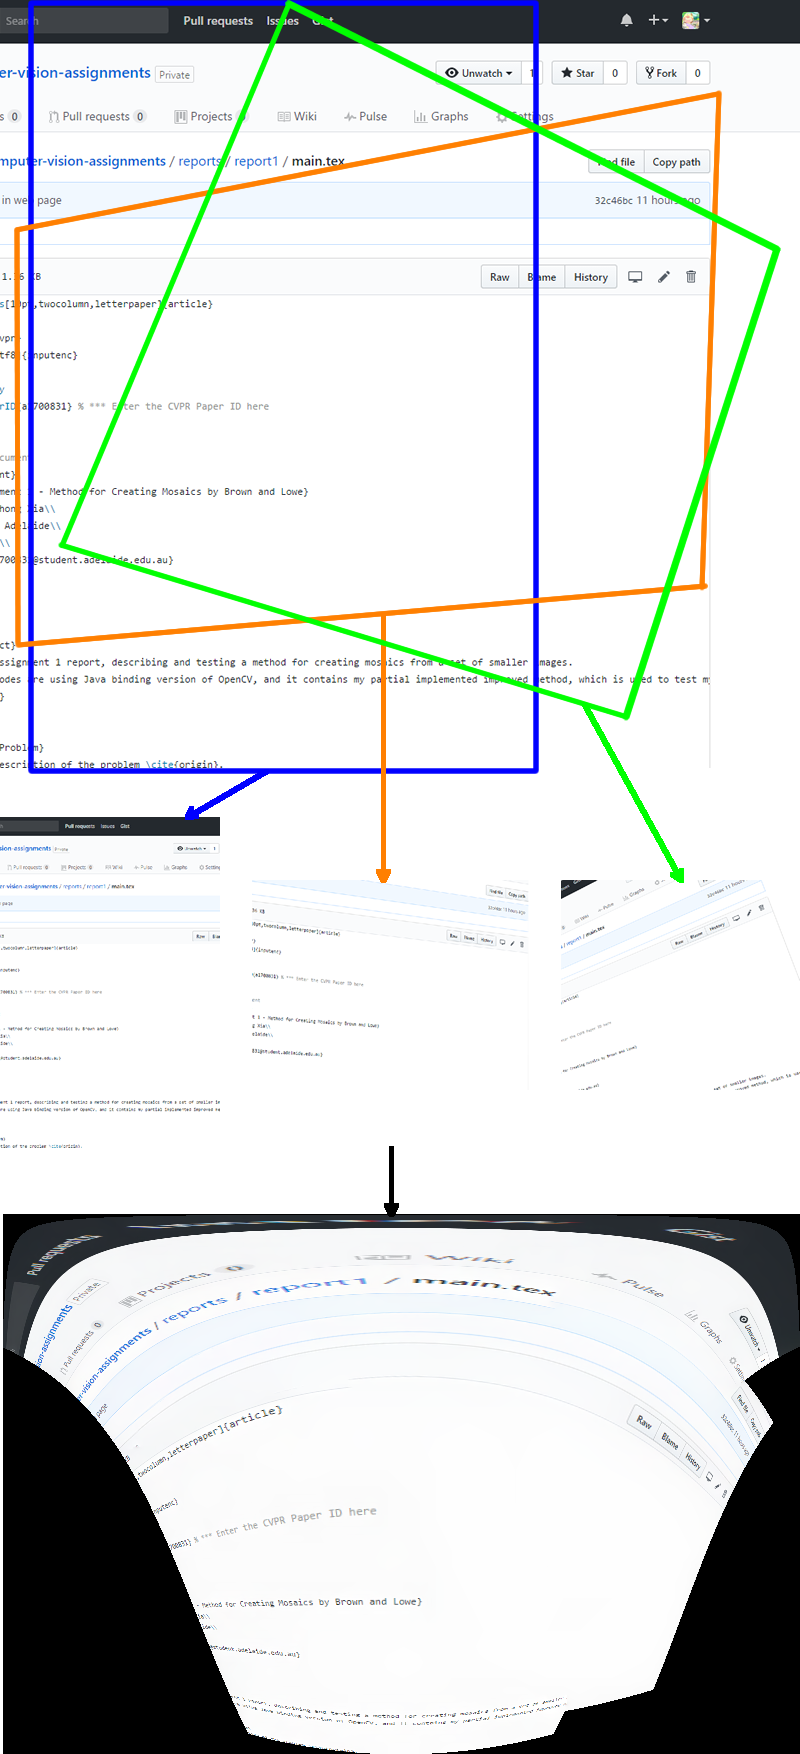
\includegraphics[width=0.9\linewidth]{fail}
    \end{center}
    \caption{The source image is a screenshot (plane), and the 3 images for stitching are cropped from the source image.
    Even when I tried using images with more than 70\% shared area, the result is still out of expectation.}
    \label{fig:fail}
\end{figure}

\begin{figure*}
    \begin{center}
        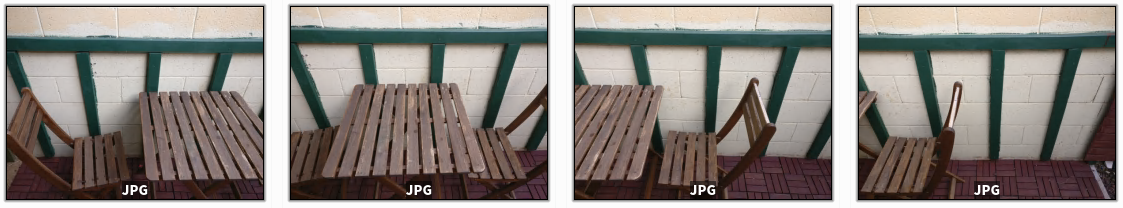
\includegraphics[width=0.9\textwidth]{horizontal_motion}
    \end{center}
    \caption{The source images are captured by horizontal moving camera, so the space projection structure is changed in every image,
    and it is impossible to match features using mentioned image matching algorithm.}
    \label{fig:cameramotion}
\end{figure*}


Hypothesis and testing, and resulting.

Anaylse the outcome of the tests, and give a useful conclusion.

\subsection{}


% Bibliography
\begin{thebibliography}{9}
\bibitem {origin}
M. Brown and D. Lowe, ``Automatic panoramic image stitching using invariant features,''
\textit{Int. J. Comput. Vision}, vol. 74, no. 1, pp. 59–73, 2007.

\bibitem {sift}
D. G. Lowe, ``Distinctive Image Features from Scale-Invariant Keypoints,''
\textit{International Journal of Computer Vision}, vol. 60, 2004.

\bibitem {knn}
Beis, J. and Lowe, D. 1997. ``Shape indexing using approximate nearest neighbor search in high-dimensional spaces,''
\textit{In Proceedings of the Interational Conference on Computer Vision and Pattern Recognition (CVPR97)}, pp. 1000–1006.

\bibitem {ransac}
Fischler, M. and Bolles, R. 1981. Random sample consensus: ``A paradigm for model fitting with application to image analysis and automated cartography'',
\textit{Communications of the ACM}, 24:381–395.

\bibitem {surf}
H., Bay, T., Tuytelaars and L., Van Gool, ``Surf: Speeded up robust features,''
\textit{Lecture Notes in Computer Science}, Vol.3951, p.404, 2006.

\end{thebibliography}

\end{document}
